\chapter{2}

\begin{task}{Task A}
	\textbf{To prove: }

	\emph{Let $X$ be a continuous real-valued random variable with CDF  :
		$\mathbb{R} \rightarrow [0, 1]$. Assume that $F_X$ is invertible. Then
		the random variable $Y := F_X (X) \in [0, 1]$ is uniformly distributed in
		$[0, 1]$}

	\textbf{Proof:}\\
	$F_X$ by definition can also be written as
	\begin{align}
		F_X(x) = P(X\leq x)
	\end{align}

	Define a new random variable $Y$,
	\begin{align}
		Y =F_X(X)
	\end{align}

	Y is the result of applying CDF $F_X$ to the random variable $X$. To
	prove the theorem, assume $y\in [0,1]$. So, the probablity that $Y \leq
		y$ is:
	\begin{align}
		P(Y\leq y) = P(F_X(X)\leq y)
	\end{align}

	It is assumed that $F_X(x)$ is invertible, so,
	\begin{align}
		P(Y\leq y) = P(X\leq F_X^{-1}(y))
	\end{align}

	which is basically, probablity that $X$ is less that or equal to
	$F_X^{-1}(y)$. This can be written in the CDF form, which is
	$F_X(F_X^{-1}(y))$. So,
	\begin{align}
		P(Y\leq y) = P(X\leq F_X^{-1}(y)) = F_X(F_X^{-1}(y)) = y
	\end{align}

	So,
	\begin{align}
		P(Y\leq y) = y
	\end{align}

	where $y\in [0,1]$, which is the CDF of uniform distribution in $[0,1]$.
	So, Y is a uniform distribution in $[0,1]$ regardless of $X$.
\end{task}

\begin{task}{Task B}
	According to the theorem proved above, CDF of any random variable $X$
	mapped with itself gives a uniform random variable $Y$ in $[0,1]$. So,
	let $Y\sim \text{Uniform}(0,1)$. Then for any random variable $X$,
	\begin{align}
		F_X(X) & = Y           \\
		X      & = F_X^{-1}(Y)
	\end{align}

	\textbf{Algorithm $\mathcal{A}$:}
	\begin{enumerate}
		\item Input: A sample $y$ from the uniform distribution on
		      $[0,1]$.
		\item Transformation:
		      \begin{itemize}
			      \item Apply the inverse CDF to $y$ to compute a
			            sample $u$.
			      \item Define $\mathcal{A}(u) = u = F_X^{-1}(y)$
		      \end{itemize}
		\item Output: The random variable $U = F_X^{-1}(Y)$
	\end{enumerate}

	This gives us the correct required random variables as, CDF of U is
	$F_U(u)$,
	\begin{align}
		P(U\leq u ) & = P(F_X^{-1}(Y) \leq u) \\
		F_U(u)      & =  P(Y \leq F_X(u))     \\
	\end{align}
	Since, $Y$ is a uniform random variable between 0 and 1,
	\begin{align}
		F_U(u) & =  F_Y(F_X(u)) \\
		F_U(u) & =  F_X(u)      \\
	\end{align}
	Since, for any uniform random variable $P$ between 0 and 1,
	\begin{align}
		F_P(x) = x
	\end{align}
	This proves that, $U$ and $X$ have the same CDF.
\end{task}


\begin{task}{Task C}
	The code can be found in \texttt{2c.py}. In this script, we generate
	random samples from a Gaussian distribution using the inverse transform
	sampling method. The function \texttt{sample(loc, scale)} begins by
	creating a sample, \texttt{x}, which consists of uniformly distributed
	random variables between 0 and 1, with a sample size of \texttt{N}
	(where \texttt{N} = $10^5$ or 100,000).

	These uniform samples, \texttt{x}, are then transformed into samples
	from a Gaussian (normal) distribution by passing them through the
	inverse cumulative distribution function (CDF) of the normal
	distribution, implemented via \texttt{norm.ppf}. The arguments
	\texttt{loc} and \texttt{scale} represent the mean and standard
	deviation of the Gaussian distribution, respectively. This
	transformation effectively maps the uniform samples to samples drawn
	from the specified Gaussian distribution, as demonstrated theoretically
	in previous sections.

	We then define the list \texttt{params}, which contains tuples of means
	and variances for the Gaussian distributions we wish to sample from and
	plot. For each set of parameters, the \texttt{sample()} function is
	called, and the resulting samples are stored in the \texttt{samples}
	list.

	Finally, we loop over the pairs of parameters (\texttt{params}) and
	their corresponding samples (\texttt{samples}) to create a histogram
	for each distribution. The histograms are plotted with 500 bins, and
	the density is normalized. A legend is included to indicate the mean
	(\texttt{$\mu$}) and standard deviation (\texttt{$\sigma$}) for each
	distribution.

	Below is the resulting histogram:
	\begin{figure}[H]
		\centering
		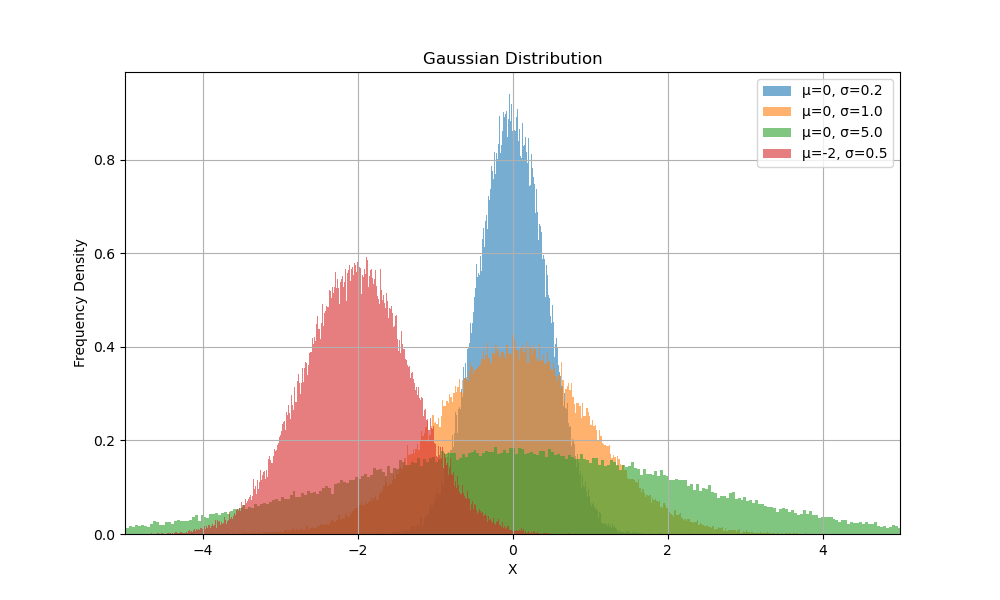
\includegraphics[width=0.8\textwidth]{../images/2c.png}
		\caption{Histograms of Gaussian distributions for different
			means and variances}
		\label{fig:gaussian_hist}
	\end{figure}
\end{task}

\begin{task}{Task D}
	The code for simulating the Galton board is found in \texttt{2d.py}. We
	implemented a function called \texttt{galton\_board}, which takes two
	parameters: \texttt{h}, representing the depth of the Galton board
	(number of pegs the ball hits), and \texttt{N}, the number of balls
	dropped.

	Inside the function, the variable steps is a matrix with \texttt{N}
	rows and \texttt{h} columns. Each row corresponds to a ball, and each
	column represents a decision the ball makes at a peg. At each step, the
	ball either moves left, represented by $-1$, or right, represented by
	$1$. The final position of each ball is determined by summing all its
	steps, which is stored in the 1-D array positions. This array records
	the final pocket into which each ball falls.

	For the simulation, $1000$ balls are dropped for different values of
	\texttt{h} (the depth of the board). The resulting distributions for
	each value of h are visualized as histograms, with the x-axis
	representing the final positions (pockets) and the y-axis showing the
	probability of balls falling into each pocket. The results for
	different values of h are shown below.
	\begin{figure}[H]
		\centering
		\begin{minipage}{0.5\textwidth}
			\centering
			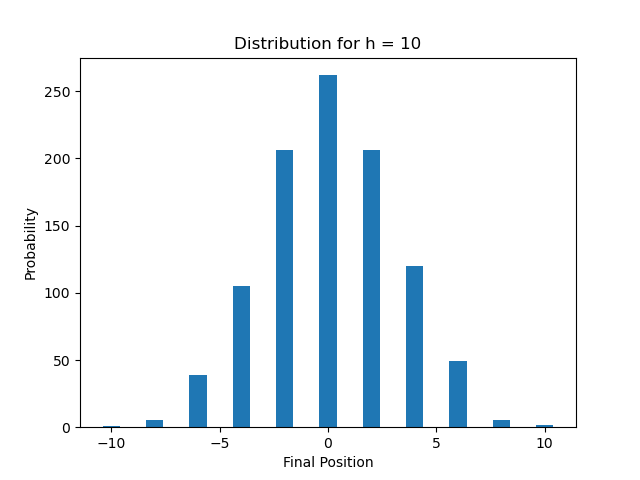
\includegraphics[width=\linewidth]{../images/2d1.png}
			\caption{Height = 10}
		\end{minipage}\hfill
		\begin{minipage}{0.5\textwidth}
			\centering
			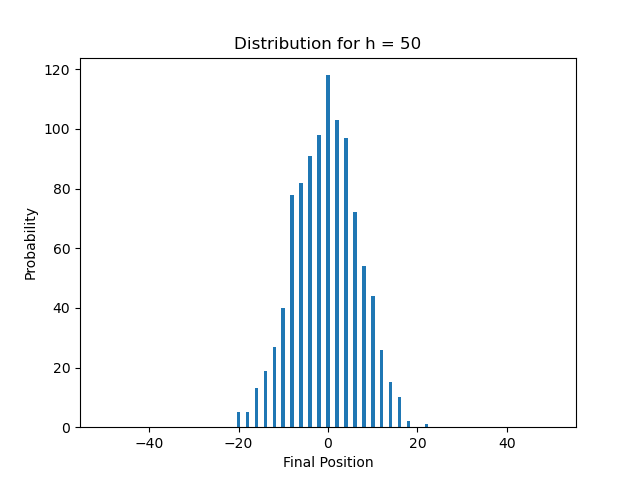
\includegraphics[width=\linewidth]{../images/2d2.png}
			\caption{Height = 50}
		\end{minipage}\hfill
	\end{figure}
	\begin{figure}[H]
		\centering
		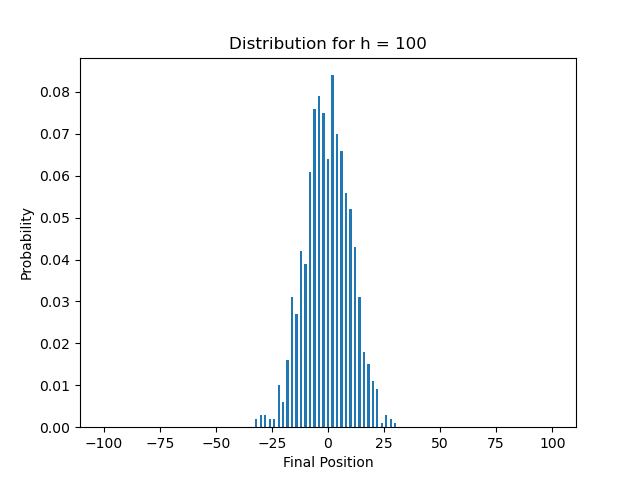
\includegraphics[width=0.8\textwidth]{../images/2d3.png}
		\caption{Height = 100}
	\end{figure}

	The shape of the tops of the histogram closely resembles a Gaussian
	distribution. As the height (\texttt{h}) of the Galton board increases,
	the distribution becomes smoother and more bell-shaped, indicating that
	most balls tend to fall around the center pockets.
\end{task}

\begin{task}{Task E(B)}
	\subsection*{- $P_h[X=2i]$ calculation}
	We have a random variable $X$ which can take values from
	$\{-h,-h+2,\ldots,h-2,h\}$. Each ball makes $h$ random binary
	decisions(left or right) as it descends. If we let $Y$ be the number of
	times the ball moves right, the final position of the ball will be
	given by,
	\begin{align}
		X = -h+2Y
	\end{align}

	where $Y$ is a \textbf{binomial variable} because in simple terms it is
	the summation of $h$ bernoulli decisions each with probability
	$\frac{1}{2}$.
	\begin{align}
		Y \sim \Bin(h,\frac{1}{2})
	\end{align}

	For a particular pocket $X = 2i$, the corresponding value of Y is:
	\begin{align}
		Y = \frac{h+2i}{2}
	\end{align}

	Thus, the probability that the ball lands in the pocket $X=2i$ is the
	probability that $Y = \frac{h+2i}{2}$. Using Binmial distribution, this
	is:
	\begin{align}
		P_h[X=2i]=P_h\left[Y=\frac{h+2i}{2}\right]=\binom{h}{\frac{h+2i}{2}}\left(\frac{1}{2}\right)^h
	\end{align}

	\subsection*{-$P_h[X=i]$ approximates to normal distribution }
	Now, we need to show $P_h[X=i]$ approximates to normal distribution for very large $h$.\\
	Using \textbf{Stirling's approximation} for large $n$, which states that:
	\begin{align}
		n!\approx \sqrt[]{2\pi n}\left(\frac{n}{2}\right)^n
	\end{align}
	$P_h$ in terms of $k$ can be written as
	\begin{align}
		P_h[X=i] = \binom{2k}{k+\frac{i}{2}}\left(\frac{1}{2}\right)^{2k}
	\end{align}
	Where $h=2k$. Let $j=\frac{i}{2}$. So, $j\in\{-k,-k+1,\ldots,k-1,k\}$. So now,

	\begin{align}
		P_h[X=2j] =  \binom{2k}{k+j}\left(\frac{1}{2}\right)^{2k}
	\end{align}

	Using Stirling's approximations,
	\begin{align}
		P_h[X=i] & = \frac{(2k)!}{(k+j)!(k-j)!}\left(\frac{1}{2}\right)^{2k} \\
		         & \approx
		\frac{\sqrt[]{2\pi(2k)}\left(\frac{2k}{e}\right)^{2k}}{\sqrt[]{2\pi(k+j)}\left(\frac{k+j}{e}\right)^{k+j}\sqrt[]{2\pi(k-j)}\left(\frac{k-j}{e}\right)^{k-j}}\left(\frac{1}{2}\right)^{2k}
		\\
		         & = \frac{\sqrt[]{4\pi k}}{\sqrt[]{2\pi
				(k+j)}\sqrt[]{2\pi (k-j)}}
		\left(\frac{2k}{e}\right)^{2k}\left(\frac{e}{k+j}\right)^{k+j}\left(\frac{e}{k-j}\right)^{k-j}\left(\frac{1}{2}\right)^{2k}
		\\
		         & = \frac{\sqrt[]{k}}{\sqrt[]{\pi
				(k+j)(k-j)}}\left(\frac{2^{2k}\cdot
			e^{k+j+k-j}}{e^{2k}\cdot2^{2k}}\right)
		\left(\frac{k^{2k}}{(k+j)^{k+j}\cdot
		(k-j)^{k-j}}\right)                                                  \\
		         & = \frac{\sqrt[]{k}}{\sqrt[]{\pi
				(k^2-j^2)}}\left(\frac{(k-j)^j}{(k+j)^j}\right)\left(\frac{k^2}{(k+j)(k-j)}\right)^k
		\\
		         & = \frac{\sqrt[]{k}}{\sqrt[]{\pi
				(k^2-j^2)}}\left(\frac{k^j\left(1-\frac{j}{k}\right)^j}{k^j\left(1+\frac{j}{k}\right)^j}\right)\left(\frac{k^2}{k^2-j^2}\right)^k
	\end{align}
	As $i \ll \sqrt[]{h}$, so $j\ll \sqrt[]{h}$ and as $h=2k$, so $j\ll
		\sqrt[]{k}$ and $j\ll k$. \\
	I will use the following well known approximation in my proof next:
	\begin{align}
		[(1+x)^n \approx 1+nx
	\end{align}
	where $x$ is close to 0.
	\begin{align}
		P_h[X=i] & = \frac{\sqrt[]{k}}{\sqrt[]{\pi
				(k^2-j^2)}}\left(1-\frac{j^2}{k}\right)\left(1-\frac{j^2}{k}\right)\left(\frac{k^2-j^2+j^2}{k^2-j^2}\right)^k
		\\
		         & = \frac{\sqrt[]{k}}{\sqrt[]{\pi
				(k^2-j^2)}}\left(1-\frac{2j^2}{k}\right)\left(1+\frac{j^2}{k^2-j^2}\right)^k
		\\
	\end{align}
	We are going to use few more well known approximation. We know that:
	\begin{align}
		\lim_{x\to \infty y\to 0} (1+y)^x = e^{xy}
	\end{align}
	\begin{align}
		\lim_{y\to 0}e^y \approx 1+y
	\end{align}
	The second approximation comes from taylor series.
	Continuing the proof:
	\begin{align}
		P_h[X=i] & = \frac{\sqrt[]{k}}{\sqrt[]{\pi (k^2-j^2)}}
		e^{\frac{-2j^2}{k}}e^{k\cdot{\frac{j^2}{k^2-j^2}}}     \\
	\end{align}
	Since $j\ll k$, $j^2 \ll k^2$, we can write $k^2-j^2=k^2$
	\begin{align}
		P_h[X=i] & = \frac{\sqrt[]{k}}{\sqrt[]{\pi
		k^2}}e^{\frac{-2j^2}{k}}e^{k\cdot{\frac{j^2}{k^2}}}     \\
		         & = \frac{1}{\sqrt[]{\pi
				k}}e^{\frac{-2j^2}{k}+\frac{j^2}{k}}
		\\
		         & = \frac{1}{\sqrt[]{\pi k}}e^{\frac{-j^2}{k}}
	\end{align}
	Substituting back the value of $j = \frac{i}{2}$
	\begin{align}
		P_h[X=i] & = \frac{1}{\sqrt[]{\pi k}}e^{\frac{-i^2}{4k}}
	\end{align}

	%  We can convert the factorials in the binomial coefficient:
	%  \begin{align}
	%  	\binom{h}{r} = \frac{h!}{r!(h-r)!}
	%  \end{align}
	% Using stirlings approximation, we have,
	% \begin{align}
	% 	\binom{h}{y} \approx \frac{\sqrt[]{2\pi
	% 	h}\left(\frac{h}{e}\right)^h}{\sqrt[]{2\pi
	% 	y}\left(\frac{y}{e}\right)^y\cdot
	% 	\sqrt[]{2\pi(h-y)}\left(\frac{h-y}{e}\right)^{h-y}}
	% \end{align}
	%  where $y = \frac{h+2i}{2}$
	% For large $h$, we can simplify this assuming small $j$ (relative to
	% $h$). In particular, $\frac{h+2i}{2}$ can be written as
	% $\frac{h}{2}$, leading to:
	% \begin{align}
	% 	\binom{h}{\frac{h+2i}{2}} \approx \frac{2^h}{\sqrt[]{\pi
	% 	h}}e^{-\frac{2i^2}{h}}
	% \end{align}
	% Substituting it back in $P_h$ gives:
	% \begin{align}
	% 	P_h[X=2i]\approx \frac{2^h}{\sqrt[]{\pi
	% 	h}}e^{-\frac{2i^2}{h}}\left(\frac{1}{2}\right)^h
	% \end{align}
	% Simplifying the powers of 2 gives:
	% \begin{align}
	% 	P_h[X=2i]\approx \frac{1}{\sqrt[]{\pi h}}e^{-\frac{2i^2}{h}}
	% \end{align}
	% which is basically normal distribution with $\mu = 0$ and $\sigma^2=h/2$

\end{task}
